\documentclass[../../main.tex]{subfiles}

\begin{document}

\subsection{Einleitung}
\label{einleitung_grundlagen}

\begin{sloppypar}
Security Awareness ist Technik. Security Awareness ist Kultur. Security Awareness ist Psychologie. Security Awareness ist Kommunikation. Security Awareness ist Wissen. Security Awareness ist \dots all dies ist richtig. \citeauthor{helisch_security_2009} (\citeyear{helisch_security_2009}) jedoch sagt:

\begin{quote}
"`\dots der Schlüssel zur Security ist unterm Strich stets der Mensch. Ihn zu verstehen, ihn zu erreichen \dots und ihn am Ende auch zu überzeugen, ihn vielleicht zu \textsc{verändern} im Sinne einer Entwicklungsgeschichte, ist die gro\ss e Aufgabe der Awareness."' (\citeauthor{helisch_security_2009} \citeyear{helisch_security_2009}, S. 7).
\end{quote}

Ohne den Faktor Mensch zu berücksichtigen greifen sämtliche Eingangs genannten Aussagen zu kurz. Security Awareness lässt sich nicht auf  technische Komponenten, psychologische Tricks oder einige clevere Kommunikationsmassnahmen reduzieren. Wohlgemerkt, diese und weitere Aspekte tragen allesamt zur Security Awareness bei, ohne sie wäre Security Awareness nicht sinnvoll umsetzbar. Was fehlt, ist jedoch der Faktor Mensch als das Bindeglied dazwischen. Der Mensch (oder aus der Firmenperspektive: die Mitarbeitenden) mit seinen komplexen, nicht immer vorhersagbaren Verhaltensmustern, seiner kulturellen Herkunft, seinem empirischen Wissens- und Erfahrungsschatz, seiner Weltanschauung und nicht zuletzt mit seinen persönlichen Bedürfnissen und Trieben ist der wichtigste und der zentrale Teil von Security Awareness.

Security Awareness an sich ist Veränderungsmanagement pur -- dieses kann aber nur tiefgreifend und nachhaltig erfolgen, wenn die "`DNA"' der Firma (Historie, Unternehmenskultur, Managementkultur, die diversen Fachkulturen, das soziale Gefüge) hinlänglich bekannt sind und in die entsprechenden Veränderungsmassnahmen miteinbezogen werden. Deshalb braucht es auch neue Ansätze, diese Veränderungen in den Arbeitsalltag und in das persönliche Lebensumfeld der Beteiligten zu integrieren (vgl. \citeauthor{helisch_security_2009} \citeyear{helisch_security_2009}, S. 7).
\end{sloppypar}

\subsection{Grundlagen und Grundsätzliche Überlegungen}

\subsubsection{OLD SCHOOL Security Awareness vs. Next Generation}
 
\begin{sloppypar}
Auf dem Sicherheitsmarkt gibt es zahlreiche Anbieter von \acrshort{cbt} Security Awareness Trainings. Die Angebote erlauben oft das Corprate Branding, sind für Kundendefinierte Anspruchsgruppen konfigurierbar, ermöglichen das Einbinden von eigenen Inhalten und bieten ein ausgefeiltes Trainee-Management System. Der Gartner Magic Quadrant 2015 für Security Awareness zeigt eine Marktübersicht der aktuellen Anbieter:
\end{sloppypar}

%% -
%% - keep this block together!!!!!!!!!!!!!!
%% - --------------------------------------
%% -
\addtocounter{figure}{1}
\begin{figure}[H]
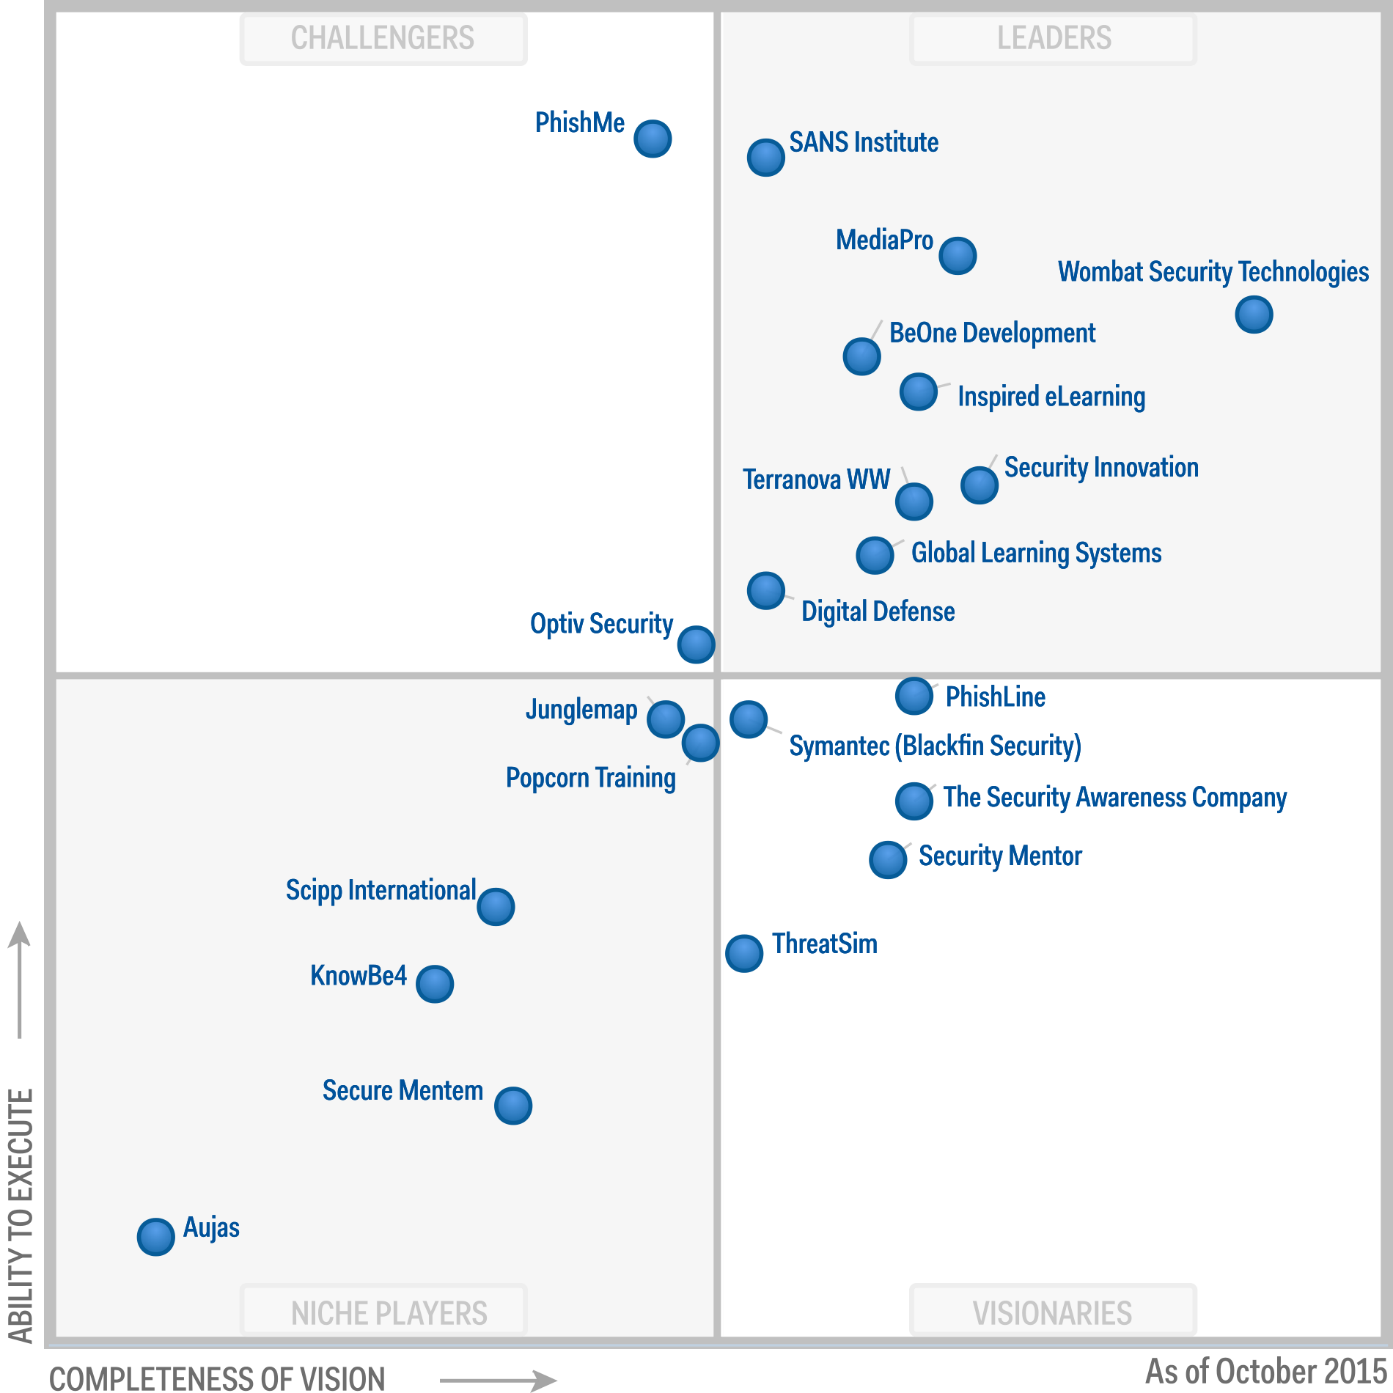
\includegraphics[width=0.5\textwidth]{Magic_Quadrant_for_SA_CBT}
\caption*{Abbildung \thefigure: Gartner Magic Quadrant für Security Awareness CBT; aus: \citeauthor{walls_magic_2015} (\citeyear{walls_magic_2015}), S. 3.}
\label{gartnermagicquadrantsecurityawarenesscbt}
\end{figure}
\addcontentsline{lof}{figure}{\numberline {\thefigure}{\ignorespaces Gartner Magic Quadrant für Security Awareness CBT}}
%% -
%% - keep this block together!!!!!!!!!!!!!!
%% - --------------------------------------
%% -

\begin{sloppypar}
Der Wert des CBT im Security Awareness Bereich ist unbestritten; wenn aber von "`Next Generation"' gesprochen werden soll, so geht die Diskussion weit über den reinen Trainingsansatz hinaus. Die typischen Merkmale von Next Generation haben einen integrierenden Charakter (vgl. \citeauthor{helisch_security_2009} (\citeyear{helisch_security_2009}), S. 8):

\begin{itemize}
\item Wenn die Massnahmen bei der Implementation unternehmenskuturell unterfüttert werden

\item Wenn die mit den Massnahmen einhergehende Veränderungmanagement die Menschen in einen Dialog miteinander bringt

\item Wenn auf bewährte Methodiken aus dem Marketing wie z.B. Wirkungsforschung zurückgegriffen wird

\item Wenn die Kommunikation der Massnahmen neue und innovative Wege beschreitet, um die Menschen zu erreichen

\item Wenn es zu den Zielen gehört, die Identifikation und die Loyalität der Mitarbeitenden gegenüber dem Unternehmen zu thematisiseren
\end{itemize}

\end{sloppypar}

\subsubsection{Wissen -- Wollen -- Können}
\label{wissen_wollen_können}
\begin{sloppypar}
Security Awareness ist keine Einzeldisziplin -- es ist vielmehr ein Zusammenspiel zwischen \textit{Wissen}, \textit{Wollen} und \textit{Können}. \citeauthor{helisch_security_2009} (\citeyear{helisch_security_2009}) sagt dazu:

\begin{quote}
"`Im Unternehmen [\dots] müssen die Mitarbeiter aber die Chance haben, das nach einer Awareness-Kampagne erworbene Sicherheitswissen sowie die Motivation, sicher handeln zu wollen, in ihrem Arbeitsumfeld dauerhaft und nachhaltig ein- und umsetzen können"' (\citeauthor{helisch_security_2009} (\citeyear{helisch_security_2009}), S. 11).
\end{quote}

Dass dabei zuerst das \textit{Wissen} als kognitiver Faktor angesprochen werden muss, liegt auf der Hand. Analogie: Erst wenn ich etwas über Sicherheit weiss, kann ich auch etwas dafür tun. 

Das \textit{Wollen} entsteht aus dem Bedürfnis heraus, die durch Wissensaufbau erfahrenen Inhalte auch anwenden zu wollen, entweder direkt am Arbeitsplatz oder durch Transportierung in das private Umfeld. Analogie: Wenn ich weiss, wie man sichere Passwörter macht, wende ich dieses Wissen auch in meinem privaten Umfeld an.

Als letzter Faktor ist das \textit{Können} zu nennen, welches vor allem auf Empowerment der Mitarbeitenden beruht. Analogie: Ich kann mich sicherheitskonform verhalten, nicht nur weil das organisatorische Umfeld dies wünscht, sondern weil es auch grundsätzlch möglich ist.

(vgl. \citeauthor{helisch_security_2009} (\citeyear{helisch_security_2009}), S. 11)
\end{sloppypar}

\end{document}